\documentclass{jarticle}
\usepackage{robomech}
\usepackage[dvipdfmx]{graphicx}

\begin{document}
\makeatletter
\title{筋骨格ヒューマノイドにおける面状牽引構造を有する膝関節の開発(仮)}
{}
{Development of Knee Joint with Planar Tract Structure on Musculoskeletal Humanoids(kari)}
{}

\author{
\begin{tabular}{lllll}
 \quad \hspace{5zw}○\hspace{1zw}鬼塚 盛宇 & (東大)&\hspace{3zw}&\quad \hspace{1zw}新城 光樹 & (東大)\\
 \quad \hspace{5zw}学\hspace{1zw}牧野 将吾 & (東大)&\hspace{3zw}& 学\hspace{1zw}河原塚 健人 & (東大)\\
 \quad \hspace{5zw}学\hspace{1zw}都築 敬 & (東大)&\hspace{3zw}& 正\hspace{1zw}浅野 悠紀 & (東大)\\
 \quad \hspace{5zw}\quad \hspace{1zw}岡田 慧 &(東大)&\hspace{3zw}& \quad \hspace{1zw}川崎 宏治 & (トヨタ自動車)\\
 \quad \hspace{5zw}正\hspace{1zw}稲葉 雅幸 & (東大) &\\
 &\\
 \multicolumn{5}{l}{\small Moritaka Onitsuka, The University of Tokyo, onitsuka@jsk.imi.i.u-tokyo.ac.jp}\\
 \multicolumn{5}{l}{\small Koki SHINJO, Shogo MAKINO, Kento KAWAHARAZUKA, Kei TSUDZUKI}\\
 \multicolumn{5}{l}{\small Yuki ASANO, Kei OKADA, Masayuki INABA, The University of Tokyo}\\
 \multicolumn{5}{l}{\small Koji KAWASAKI, TOYOTA MOTOR CORPORATION}
\end{tabular}
}
\makeatother

\abstract{
\small
Abstract will be here.
}

\date{} % 日付を出力しない
\keywords{Biomimetic Humanoid, Ligaments, Planar structure}

\maketitle
\thispagestyle{empty}
\pagestyle{empty}

\small
\section{はじめに}
筋骨格ヒューマノイド\cite{SR2017:asano:design}は人体を模した身体構造を特徴とし、骨格の周囲にアクチュエータとして筋を配置して駆動する人型ロボットである。人体の骨格に見られる柔軟な劣駆動多節構造を有する背骨や特異点の存在しない開放型球関節が実現されている上、冗長に多数取り付けられた筋によって関節の可変剛性制御を可能としている。人体模倣を規範として設計され、人と同様の巧みな身体動作が期待される。
\begin{itemize}
\item 人の筋骨格系において動作に

\item 筋骨格ヒューマノイドは骨格に取り付けられた筋が張力を発揮して骨格を牽引するという駆動方式をとっているが、人体において関節をまたいで骨格を牽引する構造としては筋の他に関節に受動的に作用する関節包や靭帯が挙げられる。両者とも関節に対して受動的に張力を発揮し、関節の安定化に貢献している。人体の関節ではこれらの受動的な骨格間牽引構造と骨格の形状によって、骨格の相対運動に拘束を設けて運動方向を決定しており、ロボットへの適用として開放型球関節の並進運動を拘束する間接包\cite{Biorob2018:fujii:capsule}や膝関節の運動を転がり曲面に拘束する靭帯\cite{RoboSym:sonoda:ligaments}についての研究などがある。
\end{itemize}
そこで本研究では骨格同士を牽引する構造として靭帯に着目し、人体における面状組織を模した構造、面状牽引構造を有する靭帯を球体関節に実装し、面状牽引構造の評価と人体の関節と同様の機能を実現する。
\section{面状牽引構造のモデル化とシミュレーション}
人体の関節はロボットの関節に比べて圧倒的に衝撃に強い。これはロボットの関節が衝撃を軸で受けるのに対し、人体の骨格は面で力を受けることができるのに加え、靭帯の受動的な張力によってソフトに支持されているからである。
\subsection{面状牽引構造}
これまで使用されてきた靭帯や筋に見られる紐や紡錘形の構造を線状牽引構造とし、骨格に対し無視できない大きさの面積を持つ構造を面状牽引構造とする。(要:定義を考える)
筋や靭帯などの骨格間牽引構造を面状にすることついては以下のような利点が挙げられる。

靭帯は紐で作られてきたが布のほうがいい。人を模した骨格の上では紐は最短経路を取ろうとするため。関節軸に対しモーメントアームが大きい曲面の極大点は基本的に不安定点で紐はそこにとどまらないが面状のそれを緩和できる。筋については面状がいいとされている\cite{Humanoids2011:osada:planar}が、靭帯については十分調べられてない。また実装上の理由として紐はロボットの骨格の隙間や突起に容易に引っかかり意図しない拘束を生じさせることがある。
\begin{itemize}
\item 大域的接触によってlocal minimaに陥らない
\item 大域的接触によって曲面の不安定点が不安定にならない。
\item 壊れにくい
\item 剛性が出しやすい
\end{itemize}
このうち剛性について述べていく。

\subsection{面状牽引構造の弾性}
\reffig{fig:schema}に線状牽引構造と面状牽引構造の比較の模式図を示す。端点が位置のみ拘束を受け回転について自由度を持つとすると、線状牽引構造は引っ張り方向(\reffig{fig:schema}のy方向)にはその弾性によって力を受けることができるが、せん断方向(\reffig{fig:schema}のx方向)は力を受けづらい。
面状牽引構造が線状牽引構造に対して剛性の面で有利であることを説明するために、シミュレーションをした。(TODO)

\begin{figure}[tb]
 \centering
  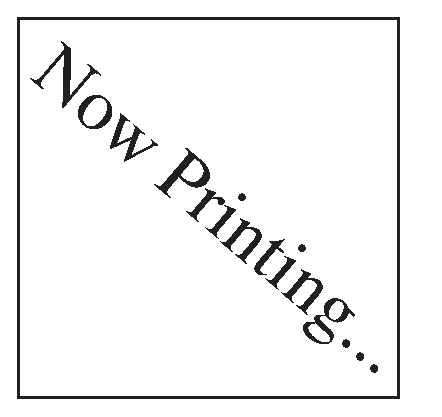
\includegraphics[height=38mm]{figs/nowprinting.eps}
  \vspace*{-4mm}
  \caption{Schematic diagram of linear tract structure and planar tract structure.}
  \label{fig:schema}
\end{figure}

\subsection{シミュレーション}
ここで得られた結果は面状構造が線状構造に対して持つ剛性における優位性を説明しており、関節に受動的な剛性を与える役割を持つ靭帯が面状である方が有利であることを示しているだけでなく、筋と骨格を結ぶ腱についても筋が与える様々な方向の張力を骨格に伝えやすいという点で腱が骨格に対して面積をもつと有利であることを示唆している。
\section{面状側副靭帯による関節受動トルクの検証}

\subsection{テストベッド}
受動的に張力を発揮して関節を保持するため、骨格に靭帯をとりつける際には張った状態で取り付けることが必要になる。Xuらの研究\cite{ICRA2011:xu:hand}では編んで作られた側副靭帯とラバースリーブによって指関節の受動的な弾性を実現しているが、作るのがめんどくさい。そこで取り付けと張力を出すのが容易な機構を作って巻き取ることで張った状態で容易に取り付けることを可能にした。
\begin{figure}[tb]
 \centering
  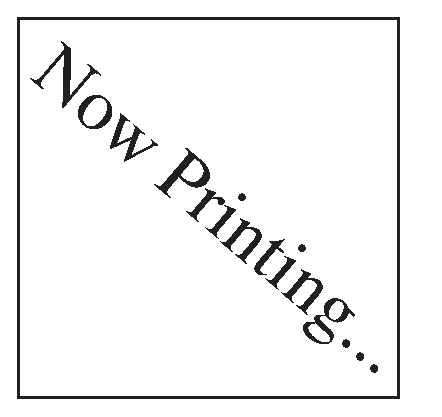
\includegraphics[height=38mm]{figs/nowprinting.eps}
  \vspace*{-4mm}
  \caption{Test bed for passive compliance by collateral ligaments.}
  \label{fig:testbed}
\end{figure}

\begin{figure}[tb]
 \centering
  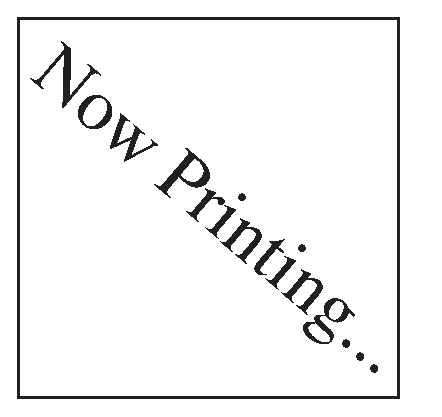
\includegraphics[height=38mm]{figs/nowprinting.eps}
  \vspace*{-4mm}
  \caption{passive compliance by collateral ligaments}
  \label{fig:passive-compliance}
\end{figure}

\subsection{膝関節への適用-終末強制回旋機構}
これまで膝の終末強制回旋機能をリジッドな機構で実現した研究\cite{IROS2013:asano:knee}がなされているが、膝伸展時に衝撃がかかることによって軸が折れるなど致命的な破壊が起きうる。人が日常しうるような衝撃を伴う動作に耐えうる関節にはソフトな拘束要素を導入することが必須であり人体では靭帯がその役割を担う。

\begin{figure}[tb]
 \centering
  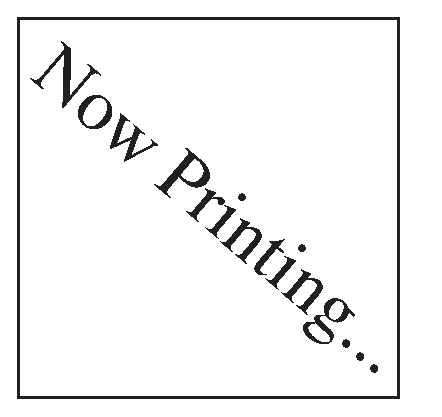
\includegraphics[height=38mm]{figs/nowprinting.eps}
  \vspace*{-4mm}
  \caption{Overview of knee joint with planar collateral ligaments.}
  \label{fig:ovv-knee}
\end{figure}

\begin{figure}[tb]
 \centering
  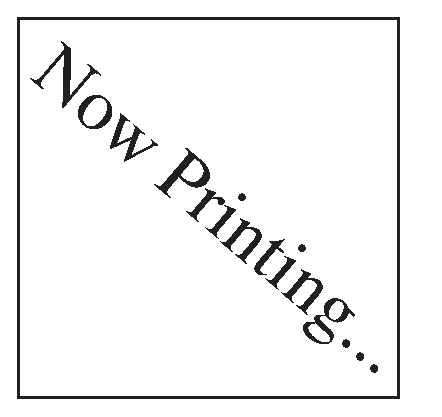
\includegraphics[height=38mm]{figs/nowprinting.eps}
  \vspace*{-4mm}
  \caption{Screw-Home movement of knee joint which angle is converged by collateral ligaments.}
  %\caption{側副靭帯による膝関節の終末回旋機能の実現}
  \label{fig:shm}
\end{figure}

\begin{figure}[tb]
 \centering
  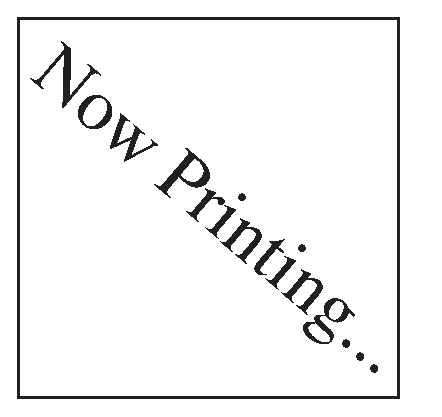
\includegraphics[height=38mm]{figs/nowprinting.eps}
  \vspace*{-4mm}
  \caption{Knee joint angle.}
  \label{fig:shm-graph}
\end{figure}

\section{結論}

\section{面状組織を付した骨格構造の今後の展開}

\footnotesize
\bibliographystyle{robomech}
\bibliography{main}

\normalsize
\end{document}
